\documentclass[10pt,a4paper]{article}
\usepackage[margin=1.7cm,top=1.6cm,bottom=1.8cm]{geometry}
\usepackage[T1]{fontenc}
\usepackage{lmodern}
\usepackage{amsmath,amssymb}
\usepackage{graphicx}
\usepackage{booktabs}
\usepackage{caption}
\usepackage{enumitem}
\usepackage{microtype}
\usepackage[hidelinks]{hyperref}
\usepackage{titlesec}
\captionsetup{font=small,labelfont=bf,skip=3pt}
\setlength{\parskip}{2.5pt plus 1pt}
\setlength{\parindent}{1em}
\setlength{\textfloatsep}{7pt plus 2pt}
\setlength{\floatsep}{6pt plus 2pt}
\setlength{\intextsep}{6pt plus 2pt}
\titlespacing*{\section}{0pt}{7pt plus 2pt}{3pt}
\titlespacing*{\subsection}{0pt}{5pt plus 2pt}{2pt}
\titleformat{\section}{\normalfont\large\bfseries}{\thesection}{0.6em}{}
\titleformat{\subsection}{\normalfont\normalsize\bfseries}{\thesubsection}{0.6em}{}
\setlist{nosep,leftmargin=1.4em}
\graphicspath{{../figures/}}
\newcommand{\Vepi}{V_{\mathrm{epi}}}

\title{\vspace{-1.2cm}\Large\bfseries Do Hopfield Episodic Memories Explain Adaptation\\ in Reversal Learning Better than Incremental RL?\vspace{-0.2cm}}
\author{Chandrani Saha (2024113002) \quad and \quad Inesh Roy (2024112015)\\[1pt]
\small Introduction to Neural and Cognitive Modelling (INCM), 2026 --- Final project report}
\date{\vspace{-0.9cm}}

\begin{document}
\maketitle

\begin{abstract}\noindent
Incremental reinforcement learning and episodic memory are two ways to adapt when the better option changes.
We implemented Q-learning (with and without choice stickiness), an episodic memory built on a modern or a
classical Hopfield network, and a hybrid of the two, and compared them on a simulated probabilistic reversal task
and on 142\,219 choices of 14 mice from the International Brain Laboratory. In simulation the building blocks
behave as theory predicts (Q-values converge; the classical network fails near $0.14N$ stored patterns; the
modern one does not), a short memory window adapts as fast as the best Q-learner, long windows and blurred
retrieval cause interference, and the models and their parameters can be recovered from choices (92.5\,\%
correct model identification). In the mice, the Hopfield memory predicts held-out choices better than
Q-learning in all 14 animals and reproduces the adaptation after block switches best, but Q-learning with
stickiness predicts individual choices at least as well (best of the four proposed models in 9 of 14 mice), and
the fitted memory is a two-trial outcome average with no similarity-based retrieval. A short outcome memory
added to stickiness gives the best account (13 of 14 mice). We find no evidence for an associative episodic
memory in this task, but clear evidence for a fast, short-lived outcome trace beyond incremental value learning.
\end{abstract}
\vspace{-0.3cm}

\section{Introduction}
Reinforcement-learning (RL) models such as Q-learning explain trial-by-trial choices as incremental updates of
option values driven by prediction errors. Animals and humans also draw on episodic memory of specific past
events when outcomes change~[7,11]. Hopfield networks are the classic model of such associative memory~[8], and
Chateau-Laurent and Alexandre~[4] showed that the differentiable dictionary of Neural Episodic Control~[12] is an
instance of the Universal Hopfield Network, which ties episodic control in RL~[3,12] to associative memory.
We ask whether a Hopfield-based episodic memory accounts for adaptation to a change in the better option
\emph{better than, or together with,} incremental RL. As proposed, the project has three parts:
(i) RL and Hopfield-memory agents are built and compared in simulation on a probabilistic reversal task;
(ii) we test whether the models can be told apart, and their parameters recovered, from choices alone;
(iii) the models are fitted to the choices of real mice from the International Brain Laboratory (IBL)~[9].
Only behaviour (choices and outcomes) is modelled. All code is our own
(Python with NumPy, SciPy and Matplotlib); the code base of~[4] was read but not copied.

\section{Methods}
\subsection{Task and models}
\textbf{Task.} In the simulated two-armed probabilistic reversal task the better arm pays with probability 0.8
and the other with 0.2; the better arm switches every 20--40 trials (uniform), and each agent plays 1000 trials.
A single \texttt{Environment} class holds the reward probabilities and the reversal schedule; with reversals
switched off it is the fixed-probability task used for the sanity check. All agents implement one interface
(\texttt{choose}, \texttt{update}), so every experiment runs unchanged on every model.
On trial $t$ the agent chooses $c_t\in\{1,2\}$ and receives $r_t\in\{0,1\}$.

\textbf{Model 1: Q-learning} ($\alpha,\theta$).
$Q_{t+1}(c_t)=Q_t(c_t)+\alpha\,(r_t-Q_t(c_t))$, $P(c_t=k)\propto e^{\theta Q_t(k)}$, $Q_1=0.5$.
\textbf{Model 2: Q-learning with perseveration} ($\alpha,\theta,\kappa$) adds a bonus for repeating the last
choice: $P(c_t=k)\propto \exp(\theta Q_t(k)+\kappa\,\mathbf 1[k=c_{t-1}])$.

\textbf{Model 3: Hopfield episodic memory} ($\beta,M,L,\theta$). After each trial one episode is stored: a key
$k_t$ (the previous $L$ choice--reward pairs, each one-hot encoded over its four possible values, all-zero for
positions before the start of the session) and a value $(c_t,r_t)$. At decision time the current history $q_t$ is
the query. In the \emph{modern} variant~[10,13] the weights over the last $M$ episodes and the value of arm $a$ are
\begin{equation}
w_i=\operatorname{softmax}_i\!\big(\beta\,k_i^{\top}q_t\big),\qquad
V(a)=\frac{\sum_i w_i\,r_i\,\mathbf 1[c_i=a]}{\sum_i w_i\,\mathbf 1[c_i=a]+\epsilon},\qquad \epsilon=10^{-6},
\label{eq:hop}
\end{equation}
and choices follow a softmax over $V$ with inverse temperature $\theta$. Here $k_i^{\top}q_t\in\{0,\dots,L\}$
counts the history positions on which episode $i$ agrees with the present situation; $\beta$ sets the retrieval
sharpness ($\beta=0$: a plain average over the window; large $\beta$: only the best-matching episodes count).
An arm with no retrievable episode has $V=0$.
In the \emph{classical} variant~[8] the last $M$ episodes are stored in a binary Hebbian network
$W=\frac1N\sum_i\xi_i\xi_i^{\top}$ (zero diagonal) over concatenated (key, choice, reward) patterns. To obtain
$\pm1$ patterns that keep the near-orthogonality of one-hot codes, each one-hot symbol is expanded into a fixed
random $\pm1$ codeword of $b$ units, the choice is coded as $\pm u$ and the reward as $\pm v$ ($u,v$ fixed random
vectors of $b$ units), so $N=(L+2)\,b$. To evaluate arm $a$ the network is cued with the key and the candidate
action, the reward units start at 0, all units are updated with $\xi\leftarrow\operatorname{sign}(W\xi)$ until
nothing changes, and $V(a)=(1+m_v)/2$ is read from the overlap $m_v$ of the reward units with $v$.

\textbf{Model 4: hybrid} ($\alpha,\theta,\beta,M,L,\lambda$): $V=(1-\lambda)\,Q+\lambda\,\Vepi$ with the modern
memory. It contains Model~1 ($\lambda=0$) and Model~3 ($\lambda=1$).

\subsection{Likelihood, fitting and recovery}
The likelihood of a choice sequence is the product of the softmax probabilities of the observed choices, each
computed from the model's values \emph{before} that trial (one-step-ahead prediction). Two implementations were
written and tested against each other to numerical precision: a literal one that replays the data through the
agent objects, and a fast exact one used for fitting (the Q-learning recursion is a linear filter per arm; for the
memory, the number and summed reward of the stored episodes per arm and match level are sufficient statistics,
so that $V$ is available for any $\beta$ at negligible cost). Gradients are analytic and were checked against
finite differences. Continuous parameters are fitted by minimising the negative log-likelihood with
\texttt{scipy.optimize} (L-BFGS-B, bounds $\alpha,\lambda\in[0,1]$, $\theta\in[0,50]$, $\beta\in[0,10]$,
$\kappa\in[-5,5]$) from many random starts. The integers $L\in\{1,2,3\}$ and $M$ (powers of two) are fitted by
an outer grid search with the continuous parameters optimised inside every cell. Because the hybrid's likelihood
has several local optima, it is additionally started from the optima of its two nested models.
This follows standard practice~[5,14]. For \textbf{recovery}~[14] we simulated 100 data sets per model with random parameters
($\alpha\sim U(0.1,0.9)$, $\theta\sim U(2,10)$, $\kappa\sim U(0.5,2)$, $\beta\sim U(0.5,4)$,
$\lambda\sim U(0.2,0.8)$, $L\in\{1,2,3\}$, $M\in\{4,8,16,32,64\}$), fitted all four models to each and selected
the winner by BIC, with $M$ and $L$ counted as free parameters.

\subsection{Real data}
\textbf{Data.} In the IBL task~[9] a grating appears on the left or right of a screen at a contrast of 100, 25,
12.5, 6.25 or 0\,\%, and the mouse is rewarded for turning a wheel towards the stimulus side. After 90 unbiased
trials, the probability that the stimulus is on the left alternates between 0.8 and 0.2 in blocks of 20--100
trials; the mouse is not told, and can use recent history to estimate this prior~[9,6]. We downloaded the
per-session trial tables of this biased-block task from the public IBL behaviour data release~[9] with the ONE
API (behaviour only). The selection was fixed in code before any model was fitted: among the mice with at least
15 biased-block sessions, laboratories were visited in alphabetical round-robin order until 15 mice were
selected, and the 15 most recent biased-block sessions of each were taken. A session was kept if it had at
least 200 completed trials and both biased block types, a mouse if it had at least 10 such sessions. One of the 15
mice had no trial tables on the server, one further session was unavailable and one was too short, which leaves
\textbf{14 mice from 9 laboratories, 208 sessions and 142\,219 trials} (6\,578--17\,845 per mouse; 80\,\% correct
overall). Trials without a response were dropped.

\textbf{Models.} As proposed, the stimulus enters every model as a logistic term and the history mechanism
predicts the remaining side bias:
\begin{equation}
P(c_t=\text{right})=\sigma\Big(\textstyle\sum_j w_j\,s_t\,\mathbf 1[|x_t|=x_j]+b+\theta\,[V_t(\text{right})-V_t(\text{left})]\Big),
\label{eq:mouse}
\end{equation}
with $x_t$ the contrast, $s_t=\pm1$ the stimulus side, one weight $w_j$ per non-zero contrast level and a constant
bias $b$ (five nuisance parameters shared by all models). The two ``arms'' are the left and right choices and
$r_t$ is the water reward, so $V$ comes from exactly the same four mechanisms (and the same code) as in the
simulation; Model~2 adds $\pm\kappa$ for the previous choice. All state is reset at the start of each session. On
a 0\,\% contrast trial only $b$ and the history term remain. This task differs from the simulated one: there the
reward probabilities of the arms reverse, here the prior over the stimulus side switches while the reward depends
on whether the choice matches the stimulus.
Besides the four models we fitted a \emph{no-history} reference (stimulus term only), the classical-memory
variant (values precomputed from the network with $N=128$; only $\theta$ is free), and, as controls not in the
proposal, Models~3 and~4 with the stickiness term of Model~2 added.

\textbf{Comparison.} For every mouse, sessions were split into five folds; each model, including $L$ and
$M\in\{2,\dots,128\}$, was fitted on four folds and scored by the log-likelihood of the held-out sessions.
(For the hybrids the continuous parameters were optimised in the six $(L,M)$ cells preferred by the nested
episodic model, to save computation.) BIC from fits to all sessions serves as a check, and a two-sided sign test
across mice compares the best model with each other one. To see the dynamics we aligned choices on 0\,\% and
6.25\,\% contrast trials to the block switches, for the mice, for the held-out model predictions, and for
simulations in which each fitted model performs the task itself on the mouse's stimulus sequence.

\section{Results}
\subsection{Step 1: each building block works on its own}
\begin{figure}[t]
\centering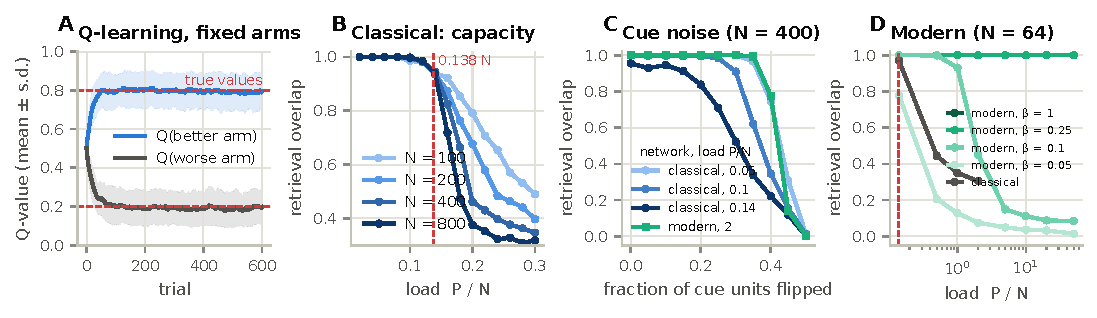
\includegraphics[width=\textwidth]{fig1_sanity.pdf}
\caption{Sanity checks. \textbf{A} Q-learning ($\alpha=0.1$, $\theta=1$, 200 runs) on a fixed 0.8/0.2 task.
\textbf{B} Classical Hopfield network: overlap between the retrieved and the stored pattern (cue with 10\,\% of
units flipped) against the load. \textbf{C} Retrieval against cue noise ($N=400$). \textbf{D} Modern network
($N=64$, 10\,\% cue noise) for four values of $\beta$, and the classical network of the same size.}
\label{fig:sanity}
\end{figure}
On a fixed-probability task the Q-values converge to the true arm values (Fig.~\ref{fig:sanity}A): averaged over
the last 100 trials they are 0.790 and 0.191 (true 0.8 and 0.2), and their spread across runs (0.091, 0.088)
equals the stationary value expected for a constant learning rate, $\sqrt{\alpha/(2-\alpha)\,p(1-p)}=0.092$.
The classical network retrieves random patterns from corrupted cues almost perfectly up to a load of
$P/N\approx0.12$ and breaks down beyond it; the transition sharpens with $N$ around the theoretical capacity
$0.138\,N$~[1] (overlap at $P/N=0.20$: 0.79, 0.68, 0.46, 0.38 for $N=100,200,400,800$; Fig.~\ref{fig:sanity}B).
Below capacity it tolerates about 30\,\% flipped cue units, less as the load grows (Fig.~\ref{fig:sanity}C).
The modern network with $\beta=1$ retrieves perfectly at every load we tried, up to $P=50N$ (3200 patterns in 64
units; the classical network of that size already fails at $P=0.5N$), and lowering $\beta$ blurs retrieval into an
average of many patterns (Fig.~\ref{fig:sanity}D), as described in~[13]. These results reproduce~[8,1,13].

\subsection{Step 2: behavioural signatures on the reversal task}
\begin{figure}[t]
\centering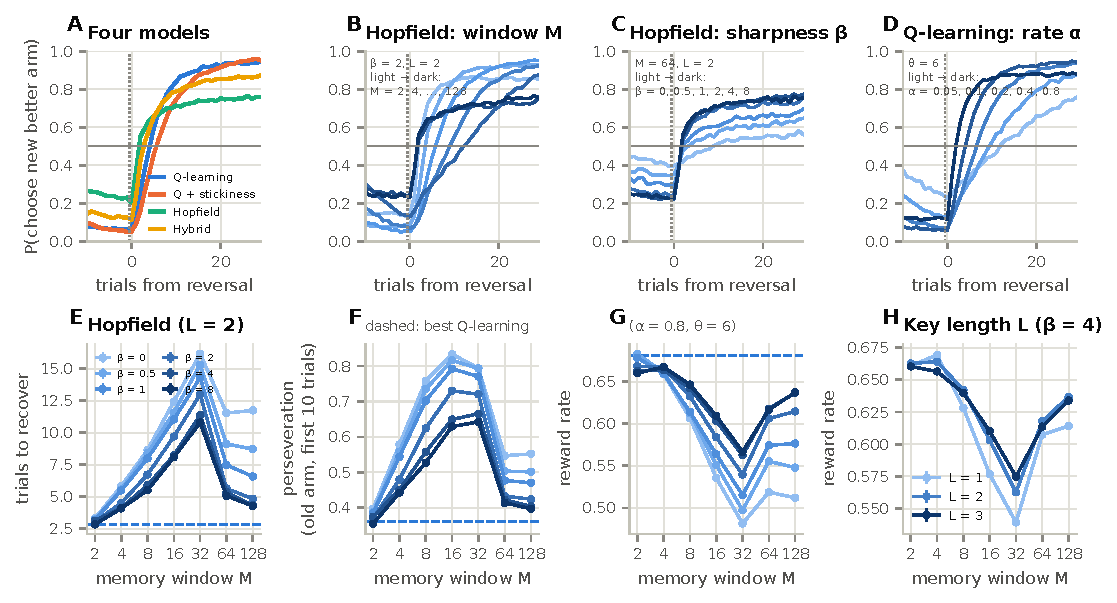
\includegraphics[width=\textwidth]{fig2_behaviour.pdf}
\caption{Reversal task, 100 sessions of 1000 trials per parameter setting ($\theta=6$ unless stated).
\textbf{A--D} Probability of choosing the new better arm around a reversal. A: Q ($\alpha=0.4$), Q+$\kappa$
($\kappa=1$), Hopfield ($\beta=4$, $M=64$, $L=2$), hybrid ($\lambda=0.5$). \textbf{E--G} Trials to recover (first
post-reversal trial that starts a run of 5 trials with at least 4 choices of the new better arm), perseveration
(fraction of old-arm choices in the first 10 trials) and reward rate of the Hopfield agent against $M$ for six
values of $\beta$ (light to dark: 0, 0.5, 1, 2, 4, 8); dashed: best Q-learner. \textbf{H} Effect of the key
length. Error bars: s.e.m.\ across sessions.}
\label{fig:behaviour}
\end{figure}
All four models adapt after a reversal, with different curve shapes (Fig.~\ref{fig:behaviour}A). For Q-learning
adaptation speed is set by $\alpha$ (trials to recover fall from 12.8 at $\alpha=0.05$ to 2.4 at $\alpha=1$), and
stickiness slows it (from 4.7 trials at $\kappa=0$ to 11.1 at $\kappa=2$).

\textbf{Prediction: small $M$ adapts faster; large $M$ or low $\beta$ causes interference.} This holds, with one
qualification. With $\beta=0$ and $L=2$, trials to recover rise from 3.3 ($M=2$) to 8.6 ($M=8$) and 16.2
($M=32$), perseveration from 0.40 to 0.79, and the reward rate falls from 0.680 to 0.481
(Fig.~\ref{fig:behaviour}B,E--G): the window still holds old-regime episodes that vote for the old arm.
Interference is worst when the window is as long as a block ($M=32$; blocks last 20--40 trials), where the
memory is out of phase with the task and the agent earns less than chance. Sharper retrieval reduces the
interference at every $M$ (at $M=32$: 16.2 trials for $\beta=0$, 10.8 for $\beta=8$). The qualification is that
for memories spanning several blocks ($M\geq64$) a sharp memory adapts quickly again (4.3 trials at $M=128$,
$\beta=8$, against 11.7 for $\beta=0$): old episodes whose key matches the current history come from the same
situation (for example, ``the last two choices of this arm were unrewarded'') and therefore carry useful rather
than interfering information. This is something an incremental learner cannot do, but it comes at the price of a
lower asymptote (Fig.~\ref{fig:behaviour}A,C). Longer keys help only at intermediate $M$
(Fig.~\ref{fig:behaviour}H). The best episodic agent is the one with the shortest memory ($M=2$, reward rate
0.687), which equals the best Q-learner ($\alpha=0.8$, $\theta=10$: 0.686); the ceiling is 0.8. In the hybrid,
adding the memory to a slow Q-learner ($\alpha=0.1$) speeds up adaptation monotonically (10.7 trials at
$\lambda=0$, 6.6 at $\lambda=0.5$).

\subsection{Capacity and noise in behaviour}
\begin{figure}[t]
\centering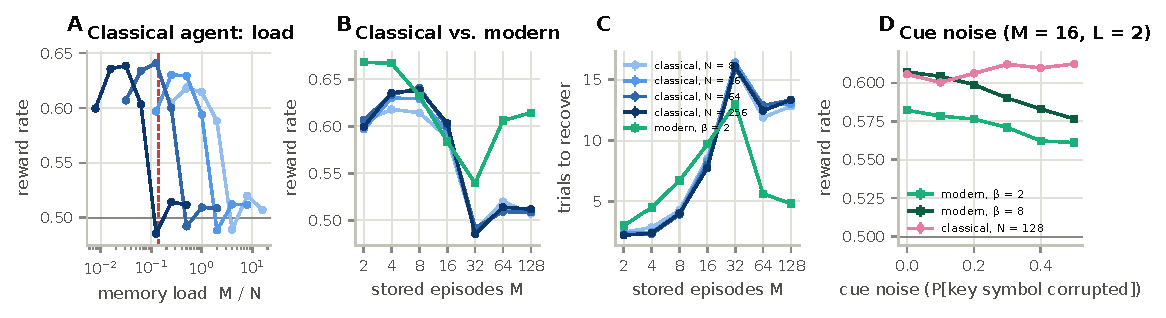
\includegraphics[width=\textwidth]{fig3_capacity_behaviour.pdf}
\caption{Agents with the classical Hebbian memory ($L=2$, $\theta=6$, 30 sessions per point; network size
$N=4b$). \textbf{A} Reward rate against the load $M/N$; dashed line: $0.138$. \textbf{B, C} The same data against
the number of stored episodes $M$, with the modern memory ($\beta=2$) for comparison. \textbf{D} Reward rate
when each symbol of the retrieval cue is replaced by a wrong one with the given probability.}
\label{fig:capacity}
\end{figure}
For the classical-memory agent we expected performance to fall once the number of stored episodes passes
$0.14N$. It does not: the reward rate depends on the number of stored episodes $M$ and not on the load $M/N$
(Fig.~\ref{fig:capacity}A,B). Networks of 8 to 256 units behave alike, all work best with 4--8 episodes
(reward rate 0.62--0.64), and all collapse to chance at $M=32$ whatever their size. The reason is that the
$0.14N$ limit is derived for random, uncorrelated patterns, whereas the episodes of this task are a handful of
distinct patterns repeated many times (at most $4^{L+1}$). Retrieval then fails through interference between
similar old and new episodes, not through a shortage of units, and enlarging the network does not help. In the
terms of~[4] the classical network weights episodes linearly by similarity, with no separation step; its curve
indeed follows the $\beta\to0$ limit of the modern memory, and unlike the sharp modern memory it does not recover
at large $M$ (Fig.~\ref{fig:capacity}B,C). The capacity limit is therefore visible at the level of patterns
(Fig.~\ref{fig:sanity}B) but is not what limits behaviour here.
Corrupting the retrieval cue lowers the reward rate of the modern agent gradually (0.607 to 0.577 for $\beta=8$
as the corruption probability goes from 0 to 0.5), towards the level of a memory that ignores the key; the
classical agent, which hardly separates episodes by key in the first place, is unaffected
(Fig.~\ref{fig:capacity}D).

\subsection{Steps 3--4: fitting and recovery}
\begin{figure}[t]
\centering
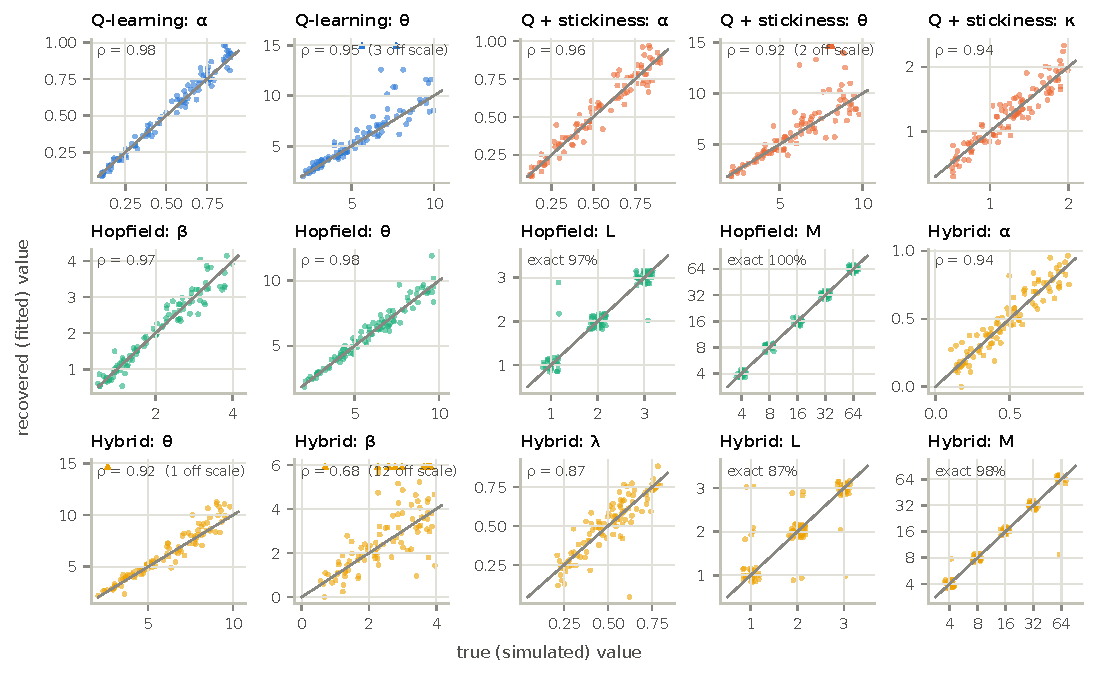
\includegraphics[width=0.62\textwidth]{fig4_parameter_recovery.pdf}\hfill
\raisebox{0.6cm}{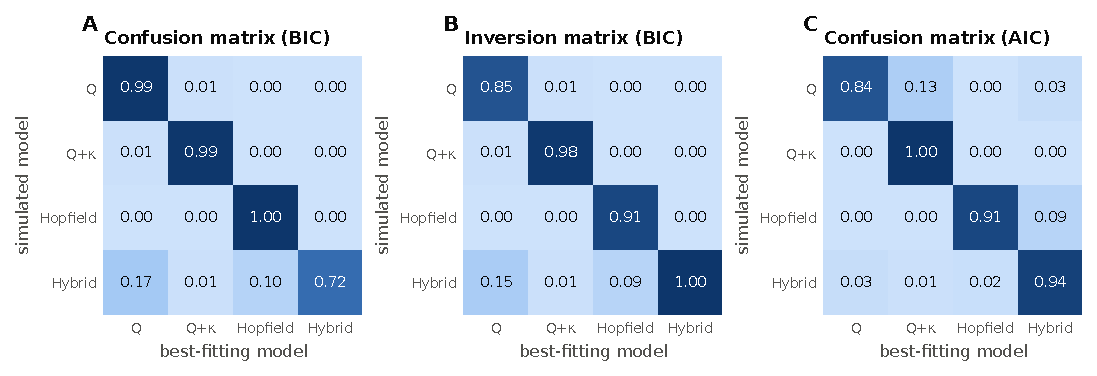
\includegraphics[width=0.36\textwidth,trim=0 0 325 0,clip]{fig5_model_recovery.pdf}}
\caption{Recovery, 100 simulated data sets per model. \textbf{Left} True against recovered parameters of the
generating model ($\rho$: Spearman correlation; integers jittered; triangles: fits beyond the plotted range).
\textbf{Right} Confusion matrix $P(\text{best-fitting model}\mid\text{simulated model})$ with BIC.}
\label{fig:recovery}
\end{figure}
The optimiser is reliable: for every model the median difference in negative log-likelihood between the random
starts was below $10^{-4}$. \textbf{Parameters are recovered} (Fig.~\ref{fig:recovery}, left): for Models~1--3
all Spearman correlations between true and fitted values are at least 0.92; the memory window is recovered
exactly in 100\,\% and the key length in 97\,\% of the Hopfield data sets. In the hybrid, $\alpha$, $\theta$,
$\lambda$ and $M$ are recovered well ($\rho=0.94$, 0.92, 0.87; $M$ exact in 98\,\%), $L$ in 87\,\%, and only the
sharpness $\beta$ is weakly identified ($\rho=0.68$). When choices are nearly deterministic $\theta$ is poorly
constrained and a few fits run to the upper bound, which lowers its Pearson (not rank) correlation.
\textbf{Models are recovered} (Fig.~\ref{fig:recovery}, right): with BIC the generating model wins in 92.5\,\%
of the 400 data sets (99, 99, 100 and 72\,\% for Models~1--4). The misses are hybrid data sets attributed to a
nested model (17\,\% to Q-learning, 10\,\% to Hopfield), which is the conservative direction for BIC; with AIC
the hybrid is recovered in 94\,\% at the cost of more false hybrids. Incremental data were never attributed to
an episodic model, and Hopfield data never to an incremental one. Reading the matrix the other way, a data set
won by Hopfield or by the hybrid was generated by an episodic model in every case. The two mechanisms can
therefore be told apart from 1000 choices, and we proceed to the real data.

\subsection{Real data: mouse choices in the IBL biased-block task}
\begin{figure}[t]
\centering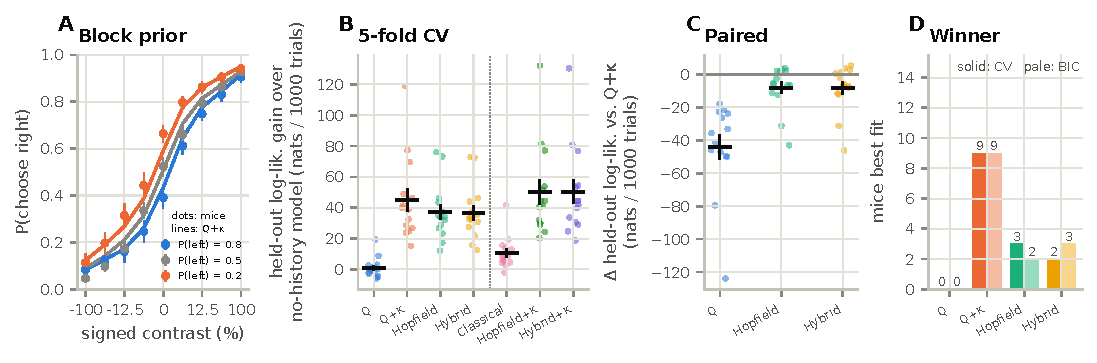
\includegraphics[width=\textwidth]{fig6_ibl_comparison.pdf}
\caption{Model comparison on 14 mice. \textbf{A} Probability of a rightward choice against signed contrast
(positive: stimulus on the right) in the three block types; dots: mice (mean $\pm$ s.e.m.\ across mice), lines:
held-out predictions of Q+$\kappa$. \textbf{B} Held-out log-likelihood of every model relative to the no-history
model; one dot per mouse, bars: mean $\pm$ s.e.m.; right of the dotted line: models that are not among the four
proposed. \textbf{C} Paired differences to Q+$\kappa$. \textbf{D} Number of mice for which each of the four
proposed models is best.}
\label{fig:iblcomp}
\end{figure}
\begin{table}[t]
\centering\small
\caption{Mouse data. $k$: free parameters including the five stimulus parameters and, for the memory models, $M$
and $L$. CV log-lik.: mean held-out log-likelihood per trial across mice. Gain: difference to the no-history
model in nats per 1000 trials (mean $\pm$ s.e.m.\ across mice). $\Delta$BIC: summed over mice, relative to the
best model. RMSE: root-mean-square difference between the simulated and the observed switch-aligned curve over
the 40 trials after a switch (Fig.~\ref{fig:iblswitch}B).}
\label{tab:ibl}
\begin{tabular}{@{}lcccccc@{}}
\toprule
Model & $k$ & CV log-lik. & Gain & Mice better than Q+$\kappa$ & $\Delta$BIC & RMSE \\
\midrule
No history (stimulus only)      & 5  & $-0.4431$ & 0              & 0/14  & 13\,300 & 0.117 \\
1\quad Q-learning               & 7  & $-0.4421$ & $1.0\pm1.7$    & 0/14  & 11\,955 & 0.103 \\
2\quad Q + stickiness           & 8  & $-0.3979$ & $45.2\pm7.3$   & --    & 1\,238  & 0.065 \\
3\quad Hopfield (modern)        & 9  & $-0.4060$ & $37.1\pm4.9$   & 5/14  & 3\,118  & 0.037 \\
4\quad Hybrid                   & 11 & $-0.4064$ & $36.8\pm4.8$   & 5/14  & 2\,854  & 0.037 \\
\midrule
3c\ \ Hopfield (classical)      & 8  & $-0.4324$ & $10.7\pm2.8$   & 0/14  & 9\,788  & 0.060 \\
\phantom{3c}\ \ Hopfield + stickiness & 10 & $-0.3930$ & $50.1\pm7.9$ & 12/14 & 198   & 0.037 \\
\phantom{3c}\ \ Hybrid + stickiness   & 12 & $-0.3929$ & $50.2\pm7.8$ & 13/14 & 0     & 0.038 \\
\bottomrule
\end{tabular}
\end{table}
The mice use the block prior: at low contrast their choices shift towards the side that is more likely in the
current block (Fig.~\ref{fig:iblcomp}A). Table~\ref{tab:ibl} and Fig.~\ref{fig:iblcomp}B--D give the comparison.

\textbf{Incremental RL alone explains almost nothing.} Q-learning improves the held-out log-likelihood over
the no-history model by only $1.0\pm1.7$ nats per 1000 trials and is better in 7 of 14 mice. In 11 mice the
fitted learning rate is below $10^{-3}$ (and $\theta$ is at its upper bound in 10), i.e.\ the values barely move
within a session. This is a property of the task, not a fitting failure: whether a choice is rewarded depends
mainly on the stimulus, so the reward value of a side carries little information about the block. The gain of Model~2 over Model~1 ($44.2$ nats per 1000 trials, 14/14 mice, sign test $p=0.0001$) is
therefore due to stickiness alone (median $\kappa=0.75$; learning rate again near zero).

\textbf{The Hopfield memory beats Q-learning but not Q-learning with stickiness.} Model~3 is better than
Model~1 in all 14 mice ($+36.1$ nats per 1000 trials, $p=0.0001$). Among the four proposed models, however,
Q+$\kappa$ has the highest mean held-out likelihood and is the best model in 9 of 14 mice, by cross-validation
and by BIC alike (Hopfield 3 and 2, hybrid 2 and 3). Its advantage over the Hopfield model ($8.1$ nats per 1000
trials, 9 of 14 mice) is not significant with the planned sign test ($p=0.42$; a Wilcoxon signed-rank test,
which also uses the size of the differences, gives $p=0.025$). The hybrid is no better than the Hopfield model
(6 of 14 mice, $p=0.79$): its Q-component is inert and it reduces to Model~3.

\textbf{What the fitted memory is.} In every mouse the Hopfield model selects the shortest window, $M=2$, and
in 12 of 14 the retrieval sharpness is $\beta=0$ (at most 0.25 in the others). With $\beta=0$ the key is not
used ($L$ is then not identified), and Eq.~\ref{eq:hop} reduces to the mean reward of each side over the last
two trials: a short-lived tendency to return to a side that was just rewarded. The data therefore give no
evidence for similarity-based retrieval of older episodes, the defining property of an associative memory; the
memory wins over Q-learning because it is fast, as the simulations predicted for small $M$. The classical
variant is clearly worse than the modern one (0 of 14 mice, $-26.4$ nats per 1000 trials) but still better than
the no-history model in 13 mice.

\textbf{Stickiness and a short outcome memory are complementary.} Since stickiness is the largest single effect,
we added it to Models~3 and~4 (not in the proposal). Both then beat Q+$\kappa$: Hopfield+$\kappa$ in 12 of 14
mice ($p=0.013$) and hybrid+$\kappa$ in 13 of 14 ($p=0.002$), by about 5 nats per 1000 trials, a ninth of the
effect of stickiness itself; the two do not differ from each other ($p=0.42$). The memory window stays short
($M=2$ or 4), and $\beta$ is 0 in 9 mice for Hopfield+$\kappa$. Summed BIC agrees (Table~\ref{tab:ibl}); per mouse it prefers
Hopfield+$\kappa$ in 9, hybrid+$\kappa$ in 4 and Q+$\kappa$ in 1.

\begin{figure}[t]
\centering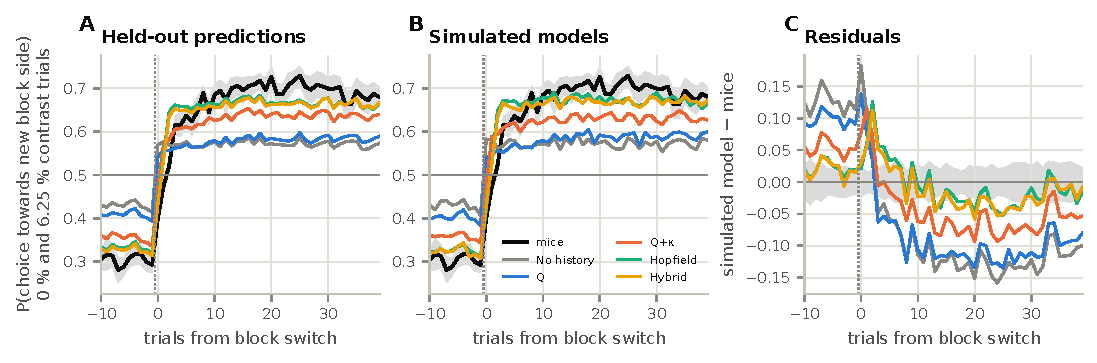
\includegraphics[width=\textwidth]{fig7_ibl_switch.pdf}
\caption{Choices around block switches on 0\,\% and 6.25\,\% contrast trials (mean across mice; shading:
s.e.m.\ of the mice). \textbf{A} Held-out one-step-ahead predictions. \textbf{B} Each fitted model performs the
task itself on the mouse's stimulus sequence (10 simulations per mouse). \textbf{C} Simulation minus mice.}
\label{fig:iblswitch}
\end{figure}
\textbf{Adaptation after a block switch.} On low-contrast trials the mice choose the side favoured by the new
block with probability 0.30 before a switch, 0.62 on the fourth trial after it and 0.70 on trials 10--39
(Fig.~\ref{fig:iblswitch}). The no-history model moves only from 0.43 to 0.57 (the weak 6.25\,\% stimuli are
themselves informative), Q-learning to 0.59 and Q+$\kappa$ to 0.63, whereas the Hopfield and hybrid models reach
0.67 and reproduce the curve best (Table~\ref{tab:ibl}, RMSE 0.037 against 0.065 for Q+$\kappa$). Stickiness
thus predicts individual choices better, while the short outcome memory accounts better for the adaptation to the
block. No model is complete: all of them stay below the mice late in the block, and the memory models switch too
abruptly (0.63--0.65 on the third trial, mice 0.52), which points to an integration over more trials than the
two-trial window that the likelihood selects.

\begin{figure}[t]
\centering
\begin{minipage}[c]{0.30\textwidth}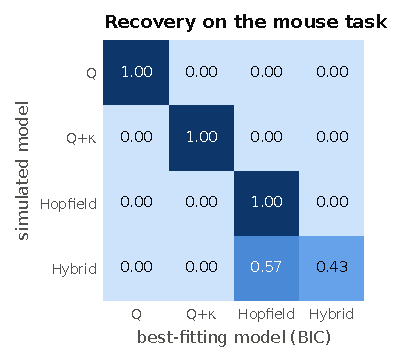
\includegraphics[width=\textwidth]{fig8_ibl_recovery.pdf}\end{minipage}\hfill
\begin{minipage}[c]{0.67\textwidth}
\caption{Model recovery under the conditions of the mouse data. For every mouse, each of the four models, with
the parameters fitted to that mouse, performed the task on the mouse's own stimulus sequence; all four models
were then fitted to the synthetic choices exactly as to the real ones. Entries:
$P(\text{best-fitting model by BIC}\mid\text{simulated model})$, 14 synthetic mice per row.}
\label{fig:iblrec}
\end{minipage}
\end{figure}
\textbf{Can the mouse fits be trusted?} The recovery analysis of Section~3.4 used the simulated task, so we
repeated it under the conditions of the real data (Fig.~\ref{fig:iblrec}). Synthetic mice generated by
Q-learning, Q+$\kappa$ and the Hopfield model were attributed to the correct model in 14 of 14 cases each, and no
incremental data set was attributed to an episodic model or vice versa. Hybrid data were attributed to the hybrid
in 6 and to the Hopfield model in 8 of 14 cases, as expected, since the fitted hybrids are almost pure Hopfield
models. The comparison between Q+$\kappa$ and the Hopfield memory in the mice is therefore not limited by the
method; the hybrid cannot be distinguished from Model~3 in these data.

\section{Discussion}
\textbf{Answer to the question.} In simulation a Hopfield episodic memory adapts to reversals as well as the
best incremental learner, and the two leave distinguishable traces in choices: the models and their parameters
can be recovered from 1000 trials. The predicted role of the memory parameters was confirmed (short windows adapt
fast, long windows and blurred retrieval interfere), with two findings we did not anticipate: a sharp memory that
spans several blocks adapts quickly again, and the behaviour of the classical network is limited by interference
between similar episodes rather than by the $0.14N$ capacity. In the mouse data the answer is mixed. The Hopfield
memory explains choices far better than incremental Q-learning in every mouse and reproduces the adaptation
after block switches best, but a Q-learner with a simple stickiness term predicts held-out choices at least as
well, and the memory that the data select is a two-trial outcome average without similarity-based retrieval.
We therefore find no evidence that mice in this task use an associative episodic memory in the sense of the
proposal; what is supported is a fast, short-lived outcome trace that adds to choice stickiness.

\textbf{Limitations.} (i) The mouse task is not a reversal task: reward depends on the stimulus, and reward
values of the two sides hardly distinguish the blocks. This penalises Q-learning on rewards, and a learner that
tracks the stimulus side or past choices (as in~[6]) would be a fairer incremental competitor; we kept the
models of the proposal. (ii) In most Q-learning fits $\theta$ is at its bound with $\alpha\approx0$, so these two
parameters are not separately interpretable in the mouse fits. (iii) The memory key contains choices and rewards
only; a key that included the stimulus might make retrieval useful. (iv) Sessions were treated as one behavioural
state; splitting them into engaged and disengaged periods~[2], an optional step of the proposal, was not done.
(v) The hybrids were optimised only in the six $(L,M)$ cells preferred by their nested memory model. (vi) We ran
several pairwise tests on 14 mice without correction; only the comparisons among the four proposed models were
planned.


\paragraph{Code and data.} All code, a README with run and data-download instructions, a demo
(\texttt{demo.py}) and the numbers behind every figure accompany this report. Every analysis is seeded and can be
re-run with the scripts \texttt{scripts/01}--\texttt{07}.

{\footnotesize
\begin{thebibliography}{99}\setlength{\itemsep}{0pt}
\bibitem{1} Amit, Gutfreund \& Sompolinsky (1985). Storing infinite numbers of patterns in a spin-glass model of neural networks. \emph{Phys.\ Rev.\ Lett.} 55, 1530.
\bibitem{2} Ashwood et al.\ (2022). Mice alternate between discrete strategies during perceptual decision-making. \emph{Nat.\ Neurosci.}
\bibitem{3} Blundell et al.\ (2016). Model-free episodic control. arXiv:1606.04460.
\bibitem{4} Chateau-Laurent \& Alexandre (2024). Relating Hopfield networks to episodic control. \emph{NeurIPS}.
\bibitem{5} Daw (2011). Trial-by-trial data analysis using computational models. In \emph{Decision Making, Affect, and Learning}, OUP.
\bibitem{6} International Brain Laboratory, Findling et al.\ (2025). Brain-wide representations of prior information in mouse decision-making. \emph{Nature} 645.
\bibitem{7} Gershman \& Daw (2017). Reinforcement learning and episodic memory in humans and animals. \emph{Annu.\ Rev.\ Psychol.} 68.
\bibitem{8} Hopfield (1982). Neural networks and physical systems with emergent collective computational abilities. \emph{PNAS} 79, 2554.
\bibitem{9} International Brain Laboratory (2021). Standardized and reproducible measurement of decision-making in mice. \emph{eLife} 10, e63711.
\bibitem{10} Krotov \& Hopfield (2016). Dense associative memory for pattern recognition. \emph{NeurIPS}.
\bibitem{11} Lengyel \& Dayan (2007). Hippocampal contributions to control: the third way. \emph{NeurIPS}.
\bibitem{12} Pritzel et al.\ (2017). Neural episodic control. \emph{ICML}.
\bibitem{13} Ramsauer et al.\ (2021). Hopfield networks is all you need. \emph{ICLR}.
\bibitem{14} Wilson \& Collins (2019). Ten simple rules for the computational modeling of behavioral data. \emph{eLife} 8, e49547.
\end{thebibliography}}

\end{document}
